% !Mode:: "TeX:UTF-8"

\chapter{结果展示}
\label{ch:results}

本章将选择DODT在KITTI追踪数据集上的一些结果进行展示,以便读者能够更好的了解DODT的性能。

\section{验证集结果展示}
\label{val_results}
本小节我们将可视化AVOD模型、Based\_DODT模型、DODT(T=1) 模型以及DODT(T=3) 模型在KITTI追踪验证数据集上的运行结果。我们将在同一个场景下绘制 AVOD与DODT(T=3) 、DODT(T=1)与DODT(T=3) 以及Based\_DODT 与 DODT(T=3)  这三对模型的对比结果,最好彩色打印查看。

\section{测试集结果展示}
\label{test_results}

本小节我们选择了KITTI追踪测试数据集中四段视频的连续四帧进行可视化,有BEV视角,3D视角以及图像视角。相同颜色表示同一辆车在不同时间的状态,最好彩色打印查看。

\begin{figure}
	\subfigure{
	\begin{minipage}[b]{0.4\linewidth}
		\begin{flushright}
			\begin{overpic}[scale=0.26]{./imgs/viz_results/06/bev/04.png}
				\put(5, 85){\color{red}{\small T = 3}}
			\end{overpic}\vspace{1pt}
			\begin{overpic}[scale=0.26]{./imgs/viz_results/06/bev/03.png}
				\put(5, 85){\color{red}{\small T = 2}}
			\end{overpic}\vspace{1pt}
			\begin{overpic}[scale=0.26]{./imgs/viz_results/06/bev/02.png}
				\put(5, 85){\color{red}{\small T = 1}}
			\end{overpic}\vspace{1pt}
			\begin{overpic}[scale=0.26]{./imgs/viz_results/06/bev/01.png}
				\put(5, 85){\color{red}{\small T = 0}}
			\end{overpic}
		\end{flushright}
	\end{minipage}}
	\subfigure{
	\begin{minipage}[b]{0.55\linewidth}
	\includegraphics[width=1\linewidth]{./imgs/viz_results/06/pc/04.png}\vspace{1pt}
	\includegraphics[width=1\linewidth]{./imgs/viz_results/06/img/04.png}\vspace{3.55pt}
	\includegraphics[width=1\linewidth]{./imgs/viz_results/06/pc/03.png}\vspace{1pt}
	\includegraphics[width=1\linewidth]{./imgs/viz_results/06/img/03.png}\vspace{3.55pt}
	\includegraphics[width=1\linewidth]{./imgs/viz_results/06/pc/02.png}\vspace{1pt}
	\includegraphics[width=1\linewidth]{./imgs/viz_results/06/img/02.png}\vspace{3.55pt}
	\includegraphics[width=1\linewidth]{./imgs/viz_results/06/pc/01.png}\vspace{1pt}
	\includegraphics[width=1\linewidth]{./imgs/viz_results/06/img/01.png}
	\end{minipage}}
	\caption{KITTI多目标追踪测试集视频片段6的一段轨迹结果。}
\end{figure}

\begin{figure}
	\centering
	\subfigure{
		\begin{minipage}[b]{0.45\linewidth}
			\begin{overpic}[scale=0.230]{./imgs/viz_results/10/bev/04.png}
				\put(5, 55){\color{red}{\small T = 3}}
			\end{overpic}\vspace{4pt}
			\begin{overpic}[scale=0.230]{./imgs/viz_results/10/bev/03.png}
				\put(5, 55){\color{red}{\small T = 2}}
			\end{overpic}\vspace{4pt}
			\begin{overpic}[scale=0.230]{./imgs/viz_results/10/bev/02.png}
				\put(5, 55){\color{red}{\small T = 1}}
			\end{overpic}\vspace{4pt}
			\begin{overpic}[scale=0.230]{./imgs/viz_results/10/bev/01.png}
				\put(5, 55){\color{red}{\small T = 0}}
			\end{overpic}
	\end{minipage}}
	\subfigure{
		\begin{minipage}[b]{0.47\linewidth}
			\includegraphics[width=1\linewidth]{./imgs/viz_results/10/pc/04.png}\vspace{1pt}
			\includegraphics[width=1\linewidth]{./imgs/viz_results/10/img/04.png}\vspace{2.5pt}
			\includegraphics[width=1\linewidth]{./imgs/viz_results/10/pc/03.png}\vspace{1pt}
			\includegraphics[width=1\linewidth]{./imgs/viz_results/10/img/03.png}\vspace{2.5pt}
			\includegraphics[width=1\linewidth]{./imgs/viz_results/10/pc/02.png}\vspace{1pt}
			\includegraphics[width=1\linewidth]{./imgs/viz_results/10/img/02.png}\vspace{2.5pt}
			\includegraphics[width=1\linewidth]{./imgs/viz_results/10/pc/01.png}\vspace{1pt}
			\includegraphics[width=1\linewidth]{./imgs/viz_results/10/img/01.png}
	\end{minipage}}
	\caption{KITTI多目标追踪测试集视频片段10的一段轨迹结果。}
\end{figure}

\begin{figure}
	%\centering
	\subfigure{
	\begin{minipage}[b]{0.4\linewidth}
	\begin{flushright}
		\begin{overpic}[trim={0cm, 3cm, 0cm, 0cm}, clip, scale=0.22]{./imgs/viz_results/11/bev/04.png}
			\put(5, 88){\color{red}{\small T = 3}}
		\end{overpic}\vspace{3pt}
		\begin{overpic}[trim={0cm, 3cm, 0cm, 0cm}, clip, scale=0.22]{./imgs/viz_results/11/bev/03.png}
			\put(5, 88){\color{red}{\small T = 2}}
		\end{overpic}\vspace{3pt}
		\begin{overpic}[trim={0cm, 3cm, 0cm, 0cm}, clip, scale=0.22]{./imgs/viz_results/11/bev/02.png}
			\put(5, 88){\color{red}{\small T = 1}}
		\end{overpic}\vspace{3pt}
		\begin{overpic}[trim={0cm, 3cm, 0cm, 0cm}, clip, scale=0.22]{./imgs/viz_results/11/bev/01.png}
			\put(5, 88){\color{red}{\small T = 0}}
		\end{overpic}
	\end{flushright}
	
	\end{minipage}}
	\subfigure{
	\begin{minipage}[b]{0.5\linewidth}
	\includegraphics[trim={0cm, 5.5cm, 0cm, 0cm}, clip,width=0.85\linewidth]{./imgs/viz_results/11/pc/04.png}\vspace{1pt}
	\includegraphics[width=0.85\linewidth]{./imgs/viz_results/11/img/04.png}\vspace{1.5pt}
	\includegraphics[trim={0cm, 5.5cm, 0cm, 0cm}, clip,width=0.85\linewidth]{./imgs/viz_results/11/pc/03.png}\vspace{1pt}
	\includegraphics[width=0.85\linewidth]{./imgs/viz_results/11/img/03.png}\vspace{1.5pt}
	\includegraphics[trim={0cm, 5.5cm, 0cm, 0cm}, clip,width=0.85\linewidth]{./imgs/viz_results/11/pc/02.png}\vspace{1pt}
	\includegraphics[width=0.85\linewidth]{./imgs/viz_results/11/img/02.png}\vspace{1.5pt}
	\includegraphics[trim={0cm, 5.5cm, 0cm, 0cm}, clip,width=0.85\linewidth]{./imgs/viz_results/11/pc/01.png}\vspace{1pt}
	\includegraphics[width=0.85\linewidth]{./imgs/viz_results/11/img/01.png}
	\end{minipage}}
	\caption{KITTI多目标追踪测试集视频片段11的一段轨迹结果。}
\end{figure}


\begin{figure}
	\centering
	\subfigure{
	\begin{minipage}[b]{0.42\linewidth}
	\begin{flushright}
		\begin{overpic}[scale=0.221]{./imgs/viz_results/12/bev/04.png}
			\put(5, 87){\color{red}{\small T = 3}}
		\end{overpic}\vspace{3pt}
		\begin{overpic}[scale=0.221]{./imgs/viz_results/12/bev/03.png}
			\put(5, 87){\color{red}{\small T = 2}}
		\end{overpic}\vspace{3pt}
		\begin{overpic}[scale=0.221]{./imgs/viz_results/12/bev/02.png}
			\put(5, 87){\color{red}{\small T = 1}}
		\end{overpic}\vspace{3pt}
		\begin{overpic}[scale=0.221]{./imgs/viz_results/12/bev/01.png}
			\put(5, 87){\color{red}{\small T = 0}}
		\end{overpic}
	\end{flushright}
	\end{minipage}}
	\subfigure{
	\begin{minipage}[b]{0.55\linewidth}
	\includegraphics[width=\linewidth]{./imgs/viz_results/12/pc/04.png}\vspace{1pt}
	\includegraphics[width=\linewidth]{./imgs/viz_results/12/img/04.png}\vspace{1.5pt}
	\includegraphics[width=\linewidth]{./imgs/viz_results/12/pc/03.png}\vspace{1pt}
	\includegraphics[width=\linewidth]{./imgs/viz_results/12/img/03.png}\vspace{1.5pt}
	\includegraphics[width=\linewidth]{./imgs/viz_results/12/pc/02.png}\vspace{1pt}
	\includegraphics[width=\linewidth]{./imgs/viz_results/12/img/02.png}\vspace{1.5pt}
	\includegraphics[width=\linewidth]{./imgs/viz_results/12/pc/01.png}\vspace{1pt}
	\includegraphics[width=\linewidth]{./imgs/viz_results/12/img/01.png}
	\end{minipage}}
	\caption{KITTI多目标追踪测试集视频片段12的一段轨迹结果。}
\end{figure}


% 打印时插入必要的空白页
\ifprint
	\newpage
	\thispagestyle{empty}
	\mbox{}
	
	% 避免空白页影响页码编号
	\clearpage
	\setcounter{page}{10}
\fi
